\chapter{Booleovské obvody ($BO$)}

\section{Definície a označenia}

\begin{definicia}
  Booleovský obvod $(BO)$ je konečný acyklický orientovaný graf, v
  ktorom každému vrcholu $v$ priradíme typ $\tau (v)\in \{
  B_{IN}\}\cup\{ B_0\}\cup\{ B_1\}\cup\{ B_2\}$ a hodnotu
  $\mathcal{V}(v)\in\{ 0,1\}$. Vrchol $v$, pre ktorý typ $\tau
  (v)\in\{ B_{IN}\}$, má vstupný stupeň 0 a nazývame ho vstupný
  vrchol. Vstupom pre booleovský obvod je $n$-tica rôznych vstupných
  vrcholov označených $\langle x_1,\dots ,x_n\rangle$. Vrchol $v$,
  pre ktorý typ $\tau (v)\in\{ B_i\}$, má vstupný stupeň $i$ a
  nazývame ho hradlo. Medzi hradlá typu $B_0$ patria konštanty ``0''
  a ``1'', do $B_1$ patria hradlá ``$I$'' a ``$\neg$''
  reprezentujúce booleovské funkcie identita a negácia a do $B_2$
  patria hradlá ``$\wedge$'' a ``$\vee$'' reprezentujúce booleovské
  funkcie AND a OR. Vrcholy s výstupným stupňom 0 nazývame výstupné.
  Výstupom pre booleovský obvod je $m$-tica rôznych výstupných
  vrcholov označených $\langle y_1,\dots ,y_m\rangle$.
\end{definicia}

\begin{definicia}
  Booleovský obvod so vstupom $\langle x_1,\dots ,x_n\rangle$ a
  výstupom $\langle y_1,\dots ,y_m\rangle$ počíta\linebreak funkciu
  $f:\;\{ 0,1\}^n\rightarrow \{ 0,1\}^m$ nasledovne. Každý vstupný
  vrchol $x_i$ má danú hodnotu\linebreak $\mathcal{V}(x_i)\in\{
  0,1\}$. Každé hradlo $h$ jednoznačne vyhodnotí hodnotu
  $\mathcal{V}(h)$ aplikovaním elementárnej booleovskej funkcie
  $\tau (h)$ na hodnoty vstupných vrcholov. Výsledná hodnota funkcie
  $f$ je daná $m$-ticou hodnôt výstupných vrcholov $\langle
  \mathcal{V}(y_1),\dots ,\mathcal{V}(y_m)\rangle$.
\end{definicia}

Všimnime si, že v definícii sme ohraničili počet vstupov vrchola,
ale nie počet výstupov. Takisto sme nezakázali, aby vstupný vrchol
bol zároveň výstupným.

Ak chceme pomocou modelu $BO$ definovať jazyky, je rozumné sa
obmedziť na $BO$ s jedným výstupným vrcholom, pričom slovo na
vstupe z $\{ 0,1\}^*$ akceptujeme práve vtedy, keď hodnota
výstupného vrchola bude 1. Toto so sebou prináša jednu
nepríjemnosť, pretože $BO$ má konečný počet vstupných vrcholov, a
teda je schopný akceptovať len konečné jazyky. Preto jazyky budeme
definovať pomocou triedy booleovských obvodov.

\begin{definicia}
  Nech $\{C_n\}_{n=0}^{\infty}$ je postupnosť booleovských obvodov,
  kde $BO$ $C_n$ s $n$ vstupnými a $m(n)$ výstupnými vrcholmi počíta
  funkciu $f_n:\; \{ 0,1\}^n\rightarrow\{ 0,1 \}^{m(n)}$. Túto
  postupnosť nazývame trieda booleovských obvodov $\{ C_n\}$
  počítajúca funkciu $f:\; \{ 0,1\}^*\rightarrow\{ 0,1\}^*$
  definovanú takto: $f(w)\equiv f_n(w)$ práve vtedy, keď $|w|=n$.
\end{definicia}

\begin{definicia}
  Nech $\{ C_n\}$ je trieda (postupnosť) booleovských obvodov
  počítajúca funkciu \\ $f:\; \{ 0,1\}^*\rightarrow\{ 0,1\}$, teda
  každý $BO$ má jeden výstupný vrchol. Jazyk akceptovaný triedou $\{
  C_n\}$ definujeme takto: $L(\{ C_n\})=\{ w\in\{ 0,1\}\mm
  f(w)=1\}$.
\end{definicia}

\section{Miery zložitosti}

Pre booleovské obvody definujeme nasledujúce miery zložitosti:
\begin{itemize}
  \item $DEPTH(C_n)$ = dĺžka najdlhšej cesty v obvode $C_n$
  \item $SIZE(C_n)$ = počet hradiel obvodu $C_n$
\end{itemize}

Ak predpokladáme, že čas, ktorý potrebuje hradlo na vyhodnotenie
výstupu je jedna časová jednotka, a čas potrebný na prenos
informácie medzi hradlami neuvažujeme, potom miera $DEPTH$ je
ekvivalentná časovej náročnosti výpočtu na $BO$.

\begin{priklad}
  Chceme vypočítať skalárny súčin dvoch $n$-bitových vektorov
  $(x_1,\dots ,x_n)$ a \linebreak $(y_1,\dots ,y_n)$. Vieme, že ich
  skalárny súčin vypočítame takto: $(x_1\wedge y_1)\vee\dots\vee
  (x_n\wedge y_n)$. \linebreak Príslušný $BO$ realizujúci tento
  výpočet je znázornený na obrázku \ref{bo_obr_scalsuc}a, z ktorého ľahko \linebreak
  vidieť, že $SIZE(C_n)=2n-1=O(n)$ a $DEPTH(C_n)=n=O(n)$.
\end{priklad}

\begin{priklad}
  \label{bo_prikl_2}

  Opäť chceme vypočítať skalárny súčin dvoch $n$-bitových vektorov,
  tentoraz však použijeme iný $BO$ $C_n$ (obr. \ref{bo_obr_scalsuc}b). Pri
  zachovaní rovnakého počtu hradiel sme znížili hĺbku obvodu na
  $DEPTH(C_n)=O(\log n)$.
\end{priklad}

\begin{figure}[!ht]
  \centering
  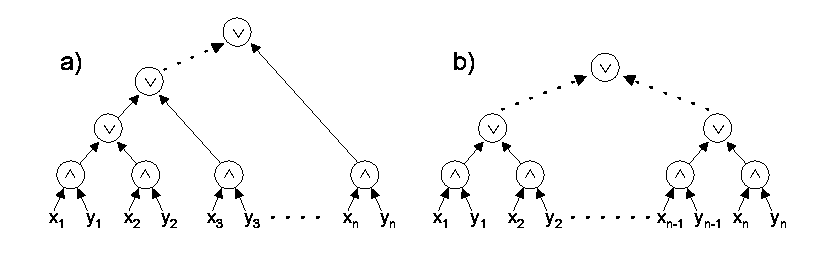
\includegraphics{img/bo/scalsuc}
  \caption{Výpočet skalárneho súčinu na $BO$} \label{bo_obr_scalsuc}
\end{figure}

\begin{priklad}
  \label{bo_prikl_3}

  Chceme vynásobiť dve booleovské matice $A$ a $B$ rozmeru $n\times
  n$. Výsledok je matica rovnakého rozmeru $C$, pričom jej prvky
  vypočítame nasledovne: $c_{i,j}=\bigvee\limits_{k=1}^{n}
  a_{ik}\wedge b_{kj}$. To je $n^2$ nezávislých skalárnych súčinov.
  Ak budeme každý takýto súčin počítať podľa príkadu
  \ref{bo_prikl_2} dostaneme príslušný obvod $C_n$, pre ktorý platí,
  že $SIZE(C_n)=O(n^3)$ a $DEPTH(C_n)=O(\log)$.
\end{priklad}

\begin{priklad}
  \label{bo_prikl_4}

  Teraz sa pokúsime vyrobiť reflexívny a tranzitívny uzáver
  booleovskej matice $M$ rozmeru $n\times n$. Výsledkom je matica
  $M^*$, ktorú dostaneme nasledovným výpočtom: \\ $M^*=I\vee M\vee
  M^2\vee\dots M^n$, kde $M^i=\bigwedge\limits_{k=1}^{i} M$, čo
  znamená, že $M^*=(I\vee M)^n$. Ak na výpočet súčinu matíc
  použijeme obvod z príkladu \ref{bo_prikl_3} a štruktúru úplného
  binárneho stromu (obr. \ref{bo_obr_tranzuzm}) dostaneme obvod $C_n$ počítajúci
  $M^*$, pre ktorý platí $SIZE(C_n)=O(n^4)$ a $DEPTH(C_n)=O(\log^2
  n)$.
\end{priklad}

\begin{figure}[!ht]
  \centering
  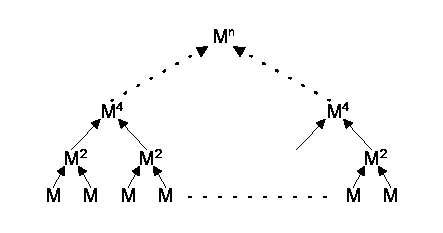
\includegraphics{img/bo/tranzuzm}
  \caption{Výpočet reflexívneho a tranzitívneho uzáveru matice} \label{bo_obr_tranzuzm}
\end{figure}

\section{$BC$-uniformné booleovské obvody}

Postupnosť booleovských obvodov, ako neskôr uvidíme, dokáže
akceptovať triedu jazykov $\mathcal{L}_{RE}$, ale tak ako sme ju
zatial zadefinovali dokáže akceptovať ešte viac, pretože
postupnosť $BO$ môžeme určiť tak, že pre rôzne dĺžky vstupu bude
používať úplne iný mechanizmus spracovania vstupného slova, čo v
iných modeloch v zásade nie je možné. Preto doterajší model $BO$
trochu zoslabíme zavedením akejsi ``pravidelnosti'' (uniformity)
do postupnosti $BO$.

\begin{definicia}
  Postupnosť booleovských obvodov je uniformná, ak existuje nejaký
  deterministický stroj ($DTS$, $ATS$), ktorý na vstupe $1^n$
  vygeneruje $BO$ $C_n$ resp. jeho kód.
\end{definicia}

\begin{definicia}
  (Štandardný kód $BO$)
  \\ Kód booleovského obvodu $C_n$ (ozn. $\langle C_n\rangle$) je postupnosť
  štvoríc $\langle g,t,a,b\rangle$, kde $g\in\{ 0,1\}^+$ je
  jednoznačné číslo vrchola, $t\in\{ 0, 1, I,\neg,\wedge,\vee, x\}$
  je typ vrchola $g$ ($x$ označuje vstup),\newline $a,b\in\{
  0,1\}^+$ sú čísla ľavého a pravého vstupu vrchola $g$. Vstupným
  vrcholom $x_1,\dots ,x_n$\linebreak štandardne priradíme čísla
  $1,\dots ,n$ a výstupnému vrcholu (ak je len jeden) priradíme
  číslo 0.
\end{definicia}

\begin{definicia}
  Postupnosť booleovských obvodov $\{ C_n\}$ je $BC$-uniformná
  ($BC$-uniformne \linebreak konštruovateľná\footnote{$BC$ -
  Borodin, Cook}), ak existuje $DTS$, ktorý pre každé $n$ na vstupe
  $1^n$ vygeneruje kód booleovského obvodu $\langle C_n\rangle$ v
  priestore\footnote{všimnime si, že pracovný priestor neurčujeme podľa veľkosti
  vstupu, ale na základe veľkosti vygenerovaného výstupu} $\log
  (SIZE(C_n))$.
\end{definicia}

\begin{figure}[!ht]
  \centering
  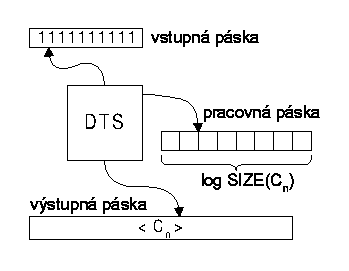
\includegraphics{img/bo/ubcdts}
  \caption{$DTS$ generujúci kód booleovského obvodu} \label{bo_obr_ubcdts}
\end{figure}

Čísla vrcholov v kóde obvodu $C_n$ kódujeme binárne, takže pre
veľkosť kódu dostávame\linebreak {$|\langle C_n\rangle|=O(SIZE(C_n).\log
SIZE(C_n))$, čo nám určuje časovú zložitosť $DTS$ z definície\linebreak
$BC$-uniformity.\\ Ďalším predpokladom na tento $DTS$ je
topologické usporiadanie výstupu t.j. kód vrchola $C_n$ sa na
výstupe neobjaví skôr ako kódy jeho vstupov.

\begin{poznamka}
  \label{bo_pozn_bcuniformita}
  $BC$-uniformita zabezpečuje len to, aby sme s jazykmi nevyšli z
  triedy $\mathcal{L}_{RE}$, teda v návrhoch postupností $BO$ nás
  príliš neobmedzuje. Preto aj každá ``rozumne'' navrhnutá
  postupnosť $BO$ je $BC$-uniformná.
\end{poznamka}

\begin{oznacenie}
  $\mathcal{U}_{BC}DEPTHSIZE(D(n),S(n))$ - trieda jazykov. Pre každý
  jazyk z tejto triedy existuje $BC$-uniformná postupnosť
  booleovských obvodov $\{ C_n\}$ akceptujúca daný jazyk pričom
  $DEPTH(C_n)=O(D(n))$ a $SIZE(C_n)=O(S(n))$.
\end{oznacenie}

\section{Porovnanie $BO$ a $TS$}

\begin{veta}
  \label{bo_veta_dtimetobosize}

  Ak $L$ je jazyk akceptovaný jednopáskovým $DTS$ v čase $T(n)$,
  potom existuje \linebreak $BC$-uniformná postupnosť $BO$ $\{
  C_n\}$ taká, že $L(\{ C_n\})=L$ a $SIZE(C_n)=O(T^2(n))$.
\end{veta}

\begin{dokaz}
  Uvažujme $DTS\; A$ a jazyk $L$ zo znenia vety. Zoberme si nejaké
  slovo $w=a_1\dots a_n\in L$. Ukážeme si ako bude vyzerať $BO$
  $C_n$ akceptujúci slová dĺžky $n$ z jazyka $L$.

  Najskôr binárne zakódujeme všetky symboly vstupnej a pracovnej
  abecedy a všetky stavy $DTS\; A$ t.j. všetkým jednoznačne
  priradíme nenulový binárny vektor. Obvod $C_n$ bude mať $T(n)$
  úrovní, pričom na $i$-tej úrovni bude ``udržiavať'' informáciu o
  $i$-tej konfigurácii $A$ pri výpočte na slove $w$ nasledovným
  spôsobom. Každá úroveň bude pozostávať z elementárnych obvodov
  $(eBO)$ reprezentujúcich jedno políčko pracovnej pásky $A$, pričom
  jeden takýto obvod dostane na vstup kód znaku, ktorý je na danom
  políčku, a kód stavu, v ktorom je $A$, ak sa hlava $A$ nachádza na
  tomto políčku (obr. \ref{bo_obr_tsboebo}a).

  Z mechanizmu výpočtu Turingovho stroja vieme, že zmeny
  konfigurácií sú len lokálneho charakteru t.j. v jednom kroku
  výpočtu sa môže zmeniť len jednopísmenkové okolie pozície hlavy.
  Podobne aj v našom obvode $C_n$ jeden elementárny obvod môže
  ovplyvniť len svojho nasledovníka a jeho susedov, preto sú
  jednotlivé elementárne obvody pospájané ako na obrázku \ref{bo_obr_tsboebo}b.

  \begin{figure}[!ht]
    \centering
    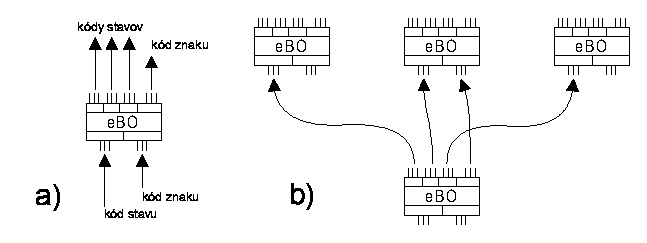
\includegraphics{img/bo/tsboebo}
    \caption{Elementárny booleovský obvod $(eBO)$} \label{bo_obr_tsboebo}
  \end{figure}

  Každý elementárny obvod bude pracovať nasledovne:
  \begin{enumerate}
    \item ak na vstup dostane kód nejakého znaku a nulový vektor ako
    kód stavu, znamená to, že hlava $A$ nie je na políčku, ktoré je
    reprezentované týmto obvodom a na výstup pošle kód prijatého znaku
    a nulový vektor ako kód stavu (obr. \ref{bo_obr_tsbo2}a)
    \item ak na vstup dostane kód znaku $a$ a kód stavu $q$, tak
    podľa definície $\delta$-funkcie $A$ pošle na výstup kód nového
    znaku $b$, a podľa pohybu hlavy v $\delta$-funkcii pošle
    príslušnému obvodu v nasledujúcej úrovni kód nového stavu, čím
    ho informuje o tom, že v nasledujúcom kroku bude hlava nad jeho
    políčkom a  ostatným dvom pošle ako kód stavu nulový vektor
    (\mbox{obr. \ref{bo_obr_tsbo2}b} pre $\delta$-funkciu $DTS$, ktorá pošle hlavu vľavo)
  \end{enumerate}

  \begin{figure}[!ht]
    \centering
    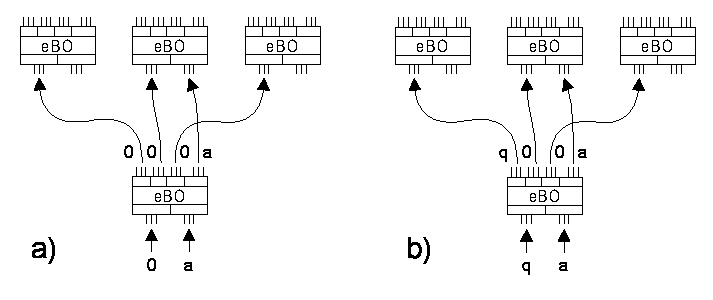
\includegraphics{img/bo/tsbo2}
    \caption{Komunikácia medzi úrovňami $eBO$} \label{bo_obr_tsbo2}
  \end{figure}

  Takže celý obvod $C_n$ bude mať $T^2(n)$ elementárnych obvodov
  ($T(n)$ úrovní pre každú kon\-fi\-gu\-rá\-ciu a v každej úrovni
  $T(n)$ obvodov pre každé políčko\footnote{v každej úrovni by
  stačilo $S(n)$ (veľkosť pracovného priestoru) obvodov, ale nemáme
  žiaden predpoklad na priestor $DTS\; A$, vieme však, že určite
  platí $S(n)\leq T(n)$ }). Vstupom pre $C_n$ bude počiatočná
  konfigurácia $A$, teda prvý obvod v prvej úrovni dostane na vstup
  kód počiatočného stavu a kód prvého písmenka slova $w=a_1\dots
  a_n$, ďalších $n-1$ obvodov dostane na vstup kódy zvyšných $n-1$
  písmenok slova $w$ a nulové vektory ako kódy stavov, a ostatné
  obvody dostanú na \mbox{vstup} nulové vektory ako kódy znakov aj
  stavov (obr. \ref{bo_obr_tsbo3}). Ďalej bude každý elementárny obvod pracovať
  ako sme už uviedli, takže jednotlivé úrovne obvodu $C_n$ budú krok
  po kroku zodpovedať konfiguráciám vo výpočte $A$. Na úrovni $T(n)$
  už iba skontrolujeme, či nejaký $eBO$ je v akceptačnom stave, ak
  áno, na výstup dáme jednotku inak nulu.

  \begin{figure}[!ht]
    \centering
    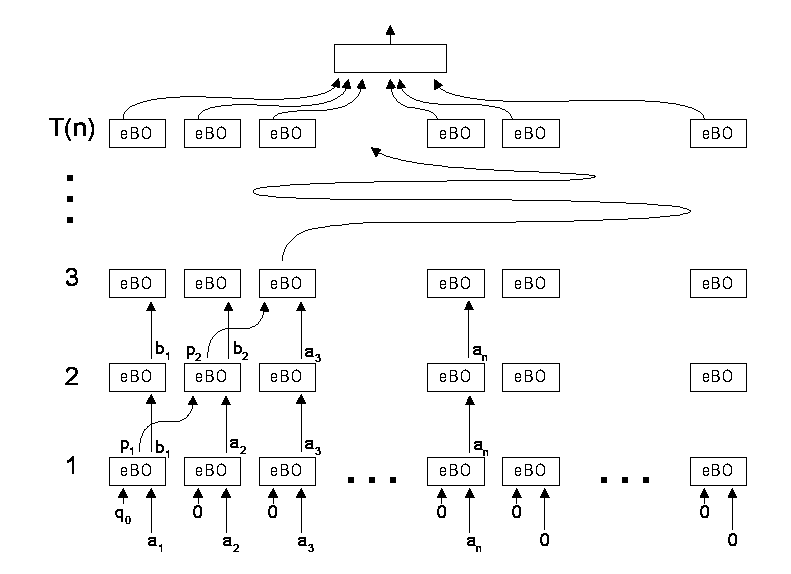
\includegraphics{img/bo/tsbo3}
    \caption{Simulácia $DTS$ booleovským obvodom} \label{bo_obr_tsbo3}
  \end{figure}

  Z uvedeného vyplýva, že $DEPTH(C_n)=T(n)$, a keďže uvažujeme
  konečný počet stavov, symbolov abecedy a konečný zápis
  $\delta$-funkcie $DTS\; A$, tak dokážeme realizovať elementárny
  obvod z konečného počtu hradiel, z čoho nakoniec plynie, že
  $SIZE(C_n)=O(T^2(n))$.

  Týmto sme ukázali, že $L\subseteq L(\{ C_n\})$. Opačná inklúzia
  (t.j. že takto zostrojená postupnosť $BO$ neakceptuje žiadne slovo
  mimo jazyka $L$) je z konštrukcie zrejmá.

  To, že takto vytvorená postupnosť $BO$ je naozaj $BC$-uniformná,
  nebudeme formálne dokazovať. Obmedzíme sa len na fakt, že každý
  obvod $C_n$ tejto postupnosti bude vytváraný rovnakým postupom, čo
  v súlade s poznámnkou \ref{bo_pozn_bcuniformita} zabezpečuje
  $BC$-unifomitu.
\end{dokaz}

\begin{veta}
  \label{bo_veta_bosizetodtime}

  Ak $L$ je jazyk akceptovaný $BC$-uniformnou postupnosťou $BO$ $\{
  C_n\}$, pričom\linebreak $SIZE(C_n)=S(n)$, potom existuje $DTS$
  akceptujúci jazyk $L$ v čase $S^3(n)$.
\end{veta}

\begin{dokaz}
  Nech $\{ C_n\}$ je postupnosť $BO$ zo znenia vety. Chceme
  zozstrojiť $DTS\; A$ taký, že $L(A)=L$. Postupnosť $\{ C_n\}$ je
  $BC$-uniformná, teda poznáme $DTS\; A'$, ktorý vygeneruje kód
  $\langle C_n\rangle$. $DTS\; A$ bude na vstupnom slove $w$ dĺžky
  $n$ pracovať nasledovne:
  \begin{enumerate}
    \item $A$ si na pásku napíše kód $BO$ $C_n$ simulovaním $A'$
    so vstupom\footnote{Takýto vstup máme k dispozícii zo vstupného
    slova $w$ tým, že všetky symboly budeme považovať za 1.} $1^n$.
    To dokáže v čase $O(S(n).\log S(n))$, lebo kód
    $\langle C_n\rangle$ je takejto dĺžky.
    \item $A$ bude postupne ohodnocovať\footnote{ohodnotiť hradlo
    znamená na páske označiť symboly príslušného hradla v kóde $C_n$
    hodnotami 0 alebo 1}
    vrcholy $BO$ $C_n$ tak, že vstupné vrcholy ohodnotí podľa
    príslušných hodnôt vstupu a hradlá ohodnotí podľa hodnôt vstupov
    hradla a jeho typu. Ohodnocovanie musí samozrejme prebiehať v topologickom
    usporiadaní. Na ohodnotenie jedného vrchola potrebuje $A$ v
    najhoršom prípade prejsť celú pásku trikrát (dvakrát na nájdenie
    hodnôt vstupov a tretí krát na nájdenie a ohodnotenie samotného
    vrchola). Vrcholov je $S(n)$, veľkosť pásky je $O(S(n).\log S(n))$,
    teda na ohodnotenie všetkých vrcholov $C_n$ potrebuje $A$ čas
    $O(S^2(n).\log S(n))$.
  \end{enumerate}
  $A$ akceptuje vstupné slovo práve vtedy, keď výstupný vrchol
  ohodnotí jednotkou. Teda ukázali sme, že $L\subseteq L(A)$. Opačná
  inklúzia je z konštrukcie zrejmá. Obidva kroky výpočtu vykoná $A$
  v čase $O(S^2(n).\log S(n))$, čo je samozrejme v $O(S^3(n))$.
\end{dokaz}

\begin{dosledok}
  $DTIME(Poly)=\mathcal{U}_{BC} SIZE(Poly)$
\end{dosledok}

\begin{dokaz}
  Z vety \ref{bo_veta_dtimetobosize} sme dostali
  $DTIME(T(n))\subseteq\mathcal{U}_{BC} SIZE(T^2(n))$.

  Z vety \ref{bo_veta_bosizetodtime} sme dostali $\mathcal{U}_{BC}
  SIZE(S(n))\subseteq DTIME(S^3(n))$.

  Spojením týchto výsledkov teda dostávame
  $DTIME(Poly)=\mathcal{U}_{BC} SIZE(Poly)$. To znamená, že vo
  výpočtovom modeli $BO$ vieme polynomiálny sekvenčný čas premieňať
  na polynomiálny paralelný priestor a opačne.
\end{dokaz}

\begin{veta}
  \label{bo_veta_nspacetobodepth}

  Ak $L$ je jazyk akceptovaný $NTS$, pracujúcim s jednou vstupnou a
  jednou pracovnou páskou, v priestore $S(n)\geq\log n$, potom
  existuje $BC$-uniformná postupnosť $BO$ $\{ C_n\}$ taká, že $L(\{
  C_n\})=L$ a $DEPTH(C_n)=O(S^2(n))$.
\end{veta}

\begin{dokaz}
  Uvažujme jazyk $L$ a $NTS\; A$ zo znenia vety. Zostrojíme $BO$
  $C_n$ akceptujúci slová dĺžky $n$ z jazyka $L$. Zoberme si nejaké
  slovo $w\in L$, kde $|w|=n$. Zamyslime sa nad tým v koľkých
  možných konfiguráciach môže byť $A$ počas výpočtu na vstupnom
  slove $w$. Ak berieme do úvahy počty stavov, symbolov abecedy,
  políčok pracovnej pásky, možné pozície hlavy na vstupnej a
  pracovnej páske, dostaneme, že počet všetkých možných konfigurácií
  je $k^{S(n)}$ pre vhodnú konštantu $k$.

  Uvažujme ďalej reláciu krok výpočtu $\vdash$ na týchto
  konfiguráciach. Za predpokladu, že binárne zakódujeme stavy a
  symboly abecedy, dokážeme reláciu $\vdash$ reprezentovať
  booleovskou maticou rozmeru $k^{S(n)}\times k^{S(n)}$, čo je pre
  pevne stanovené $n$ konečná matica. Predpokladajme, že $A$ má
  jednoznačne danú akceptačnú konfiguráciu. Potom otázka, či vstupné
  slovo $w$ patrí do jazyka $L$, je vlastne otázka, či počiatočná
  konfigurácia $A$ je v relácii $\overset{*}{\vdash}$ s akceptačnou
  konfiguráciou. Relácia $\overset{*}{\vdash}$ je reflexívnym a
  tranzitívnym uzáverom relácie $\vdash$. Keďže túto reláciu vieme
  reprezentovať konečnou booleovskou maticou, z príkladu
  \ref{bo_prikl_4} plynie, že aj reláciu $\overset{*}{\vdash}$ vieme
  reprezentovať konečnou booleovskou maticou, ktorú dostaneme
  konečným násobením mocnín matice reprezentujúcej reláciu $\vdash$.
  Z uvedeného príkladu tiež vieme, že reflexívny a tranzitívny
  uzáver booleovskej matice $M$ rozmeru $k^{S(n)}\times k^{S(n)}$
  vypočítame na $BO$ hĺbky rádovo $\log^2 k^{S(n)}=O(S^2(n))$.

  Teda náš $BO$ $C_n$ so vstupom $\langle w\rangle$ najskôr zostrojí
  maticu relácie $\vdash$ na vstupnom slove $w$ (to sa dá konečným
  $BO$, v ktorom je zakódovaná $\delta$-funkcia $A$), a potom už
  spomínaným spôsobom urobí nad touto maticou jej reflexívny a
  tranzitívny uzáver. $A$ akceptuje práve vtedy, keď vo výslednej
  matici je na i-tom riadku a j-tom stĺpci 1, kde i-ty riadok
  reprezentuje počiatočnú konfiguráciu a j-ty stĺpec reprezentuje
  akceptačnú konfiguráciu. Takto sme ukázali, že $L\subseteq L(\{
  C_n\})$, pričom $DEPTH(C_n)=O(S^2(n))$. Opačná inklúzia je z
  konštrukcie zrejmá.

  Tvrdenie o tom, že vytvorená postupnosť $BO$ je $BC$-uniformná,
  nechávame opäť na poznámku \ref{bo_pozn_bcuniformita}.
\end{dokaz}

\begin{veta}
  \label{bo_veta_bodepthtodspace}

  Ak $L$ je jazyk akceptovaný $BC$-uniformnou postupnosťou $BO$ $\{
  C_n\}$, pričom\linebreak $DEPTH(C_n)=D(n)$, potom existuje $DTS$
  akceptujúci jazyk $L$ v priestore $O(D(n))$.
\end{veta}

\begin{dokaz}
  Uvažujme jazyk $L$ a postupnosť $BO$ $\{ C_n\}$ zo znenia vety.
  Chceme zostrojiť príslušný $DTS\;A$. Nech $w\in L$ je dĺžky $n$, čiže
  kód $\langle w\rangle$ je akceptovaný $BO$ $C_n$ z postupnosti $\{
  C_n\}$. Vieme, že $\{ C_n\}$ je $BC$-uniformná, takže existuje
  generátor $A'$ kódu $\langle C_n\rangle$ pracujúci v priestore
  $\log (SIZE(C_n))$. Zrejme $\log (SIZE(C_n))\in O(D(n))$, takže $A$ má
  dostatok priestoru, aby mohol simulovať $A'$, ale nemá dosť
  priestoru na uloženie celého kódu $\langle C_n\rangle$. Nemôžeme
  teda použiť techniku ohodnocovania $C_n$ ako v dôkaze vety
  \ref{bo_veta_bosizetodtime}.

  $A$ bude postupne ohodnocovať vrcholy $C_n$ postorder
  prehľadávaním $C_n$ od výstupného vrcholu (vstupný vrchol ohodnotí
  podľa príslušnej časti vstupu $\langle w\rangle$ a vnútorný podľa
  hodnôt jeho\linebreak vstupov). $A$ však nemá na páske ani toľko
  priestoru, aby si zapamätal kódy všetkých vrcholov na ceste od
  výstupného k práve prehľadávanému vrcholu\footnote{Cesta môže byť
  dlhá maximálne $D(n)$ a kód každého vrcholu je veľkosti rádovo
  $\log SIZE(C_n)$, takže by sme potrebovali priestor rádovo $D^2(n)$.}. Preto
  si bude na páske pamätať len navigačnú cestu od výstupného k práve
  prehľadávanému vrcholu (obr. \ref{bo_obr_bots}). Ak sa chce $A$ posunúť pri
  prehľadávaní z jedného vrchola do druhého (t.j. z otca do syna
  alebo opačne), zakaždým musí spustiť simuláciu $A'$ a v jeho
  výstupe nájsť kód príslušného vrchola. Vstupné slovo $w$ bude $A$
  akceptovať práve vtedy, keď výstupný vrchol dostane hodnotu 1.

  \begin{figure}[!ht]
    \centering
    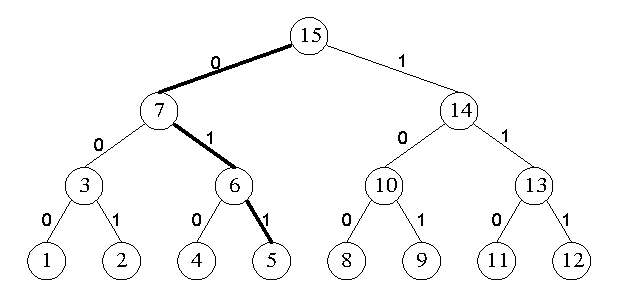
\includegraphics{img/bo/bots}
    \caption{Postorder prehľadávanie booleovského obvodu} \label{bo_obr_bots}
  \end{figure}

  Takže $A$ si bude na páske udržiavať kódy práve prehľadávaného
  vrcholu a niekoľko málo vrcholov v jeho okolí (aby mohol vrchol
  ohodnotiť), navigačnú cestu od koreňa k prehľadávanému vrcholu a
  už známe ohodnotenia vrcholov, ktoré má aktuálne na páske. Na toto
  potrebuje $A$ priestor rádovo $D(n)$. Na simulovanie $A'$
  potrebuje tiež priestor rádovo $D(n)$, takže veľkosť pracovnej
  pásky $A$ bude $O(D(n))$.

  Týmto sme ukázali, že $L\subseteq L(A)$, opačná inklúzia by opäť
  mala byť z konštrukcie zrejmá.
\end{dokaz}

\pagebreak

\begin{dosledok} \label{bo_dosl_nspacepolyubcdepthpoly}
  $NSPACE(Poly)=\mathcal{U}_{BC} DEPTH(Poly)$
\end{dosledok}

\begin{dokaz}
  Z vety \ref{bo_veta_nspacetobodepth} sme dostali
  $NSPACE(S(n))\subseteq\mathcal{U}_{BC} DEPTH(S^2(n))$.

  Z vety \ref{bo_veta_bodepthtodspace} sme dostali $\mathcal{U}_{BC}
  DEPTH(D(n))\subseteq DSPACE(D(n))$.

  Zo Savitchovej vety vieme, že $DSPACE(Poly)=NSPACE(Poly)$.

  Spojením týchto výsledkov teda dostávame
  $NSPACE(Poly)=\mathcal{U}_{BC} DEPTH(Poly)$. To\linebreak znamená,
  že vo výpočtovom modeli $BO$ vieme polynomiálny sekvenčný priestor
  premieňať na polynomiálny paralelný čas a opačne.
\end{dokaz}


\section{Druhá počítačová trieda a Nick Class}

V tejto časti si povieme nakoľko sú paralelné výpočtové modely, ktoré sme doteraz spomenuli a ktoré
ešte len spomenieme, vhodné na efektívne riešenie problémov, či je daný model vhodne zadefinovaný a
ukážeme si akými mierami budeme posudzovať vhodnosť daného modelu.

\begin{definicia}
  Model počítača patrí do druhej počítačovej triedy, ak sekvenčný nedeterministický
  priestor je v polynomiálnom vzťahu s časom na danom modeli.
\end{definicia}

Predchádzajúca definícia hovorí o tom aké kritérium sme zvolili na posudzovanie toho, či je nejaký
výpočtový model pre nás zaujímavý (vhodný). Z doteraz spomenutých modelov patria do druhej
počítačovej triedy modely Alternujúcich Turingových strojov (dôsledok
\ref{alter_dosl_nspacepolyatimepoly}) a $BC$-uniformných booleovských obvodov (dôsledok
\ref{bo_dosl_nspacepolyubcdepthpoly}).

Takmer všetky paralelné modely patria do druhej počítačovej triedy. Ak uvažujeme nejaký nový model
a chceme ho zaradiť do druhej počítačovej triedy, tak môžme urobiť simuláciu daného modelu s
Turingovým strojom podobne, ako sme to urobili vo vetách \ref{bo_veta_nspacetobodepth} a
\ref{bo_veta_bodepthtodspace}, alebo urobíme simuláciu s modelom, ktorý tam už patrí.

Ďalšou otázkou, ktorá je pre nás zaujímavá, je aké problémy môžeme považovať za efektívne paralelne
riešiteľné. Vieme, že pri sekvenčných modeloch tieto problémy tvoria triedu $\mathcal{P}$, teda sú
to problémy, ktoré vieme riešiť v polynomiálnom čase. Za efektívne riešiteľné považujeme pri
paralelných modeloch problémy patriace do triedy $\mathcal{NC}$ (Nick Class).

\pagebreak

\begin{definicia}
  Nick Class
  \begin{itemize}
    \item $\mathcal{NC}^i=\mathcal{U}_{BC}DEPTHSIZE(\log^i n,n^{O(1)})$
    \item $\mathcal{NC}=\bigcup\limits_{i\geq 1} \mathcal{NC}^i$
  \end{itemize}
\end{definicia}

Z doterajších poznatkov (pozri vety \ref{bo_veta_bosizetodtime} a \ref{bo_veta_bodepthtodspace})
vieme o práve zadefinovanej triede $\mathcal{NC}$ vysloviť pár tvrdení:

\begin{veta}
  Postavenie triedy $\mathcal{NC}$ medzi inými zložitostnými triedami.
  \begin{itemize}
    \item $\mathcal{NC}\subseteq\mathcal{P}$
    \item $\mathcal{NC}^i\subseteq DSPACE(\log^i n)$
  \end{itemize}
\end{veta}

Doterajšie teoretické výsledky ukazujú, že medzi triedami platí nasledovná hierarchia:

\centerline{$\mathcal{NC}\subseteq\mathcal{P}\subseteq\mathcal{NP}\subseteq PSPACE$}

Vieme, že $\bigcup\limits_{i\geq 1} DSPACE(\log^i n)\subset PSPACE$. Z predchádzajúcej vety
dostávame\\ $\mathcal{NC}\neq PSPACE$. Otvoreným problémom zostáva, ktorá z inklúzií v spomenutej
hierarchii tried je ostrá.

\section{Iné uniformity pre booleovské obvody}

$BC$-uniformita nie je jedinou možnosťou ako uniformovať
booleovské obvody. Niekedy sa nám táto uniformita na naše účely
nehodí. Preto teraz ukážeme ďalšie dva spôsoby ako možno
uniformovať booleovké obvody, a tie neskôr využijeme pri porovnaní
s alternujúcimi Turingovými strojmi.

\begin{definicia}
  Nech $\{ C_n\}$ je postupnosť $BO$. Jej príslušným rozšíreným
  jazykom prepojení je jazyk $L_e=\{
  \\ \langle n,g,p,y\rangle\mm
  n\in\{ 1\}^+, g\in\{ 0,1\}^+, p\in\{ L,R\}^*, |p|\leq\log
  SIZE(C_n), y\in \{ x, \wedge, \vee, \neg\}\cup\{ 0,1\}^+$, kde
  \begin{itemize}
    \item $n$ udáva\footnote{všimnime si, že $n$ je kódované unárne},
    že slovo $\langle n,g,p,y\rangle$ popisuje obvod $C_n$
    \item $g$ je binárne kódované číslo vrchola obvodu $C_n$
    \item $p$ je buď $\varepsilon$ alebo navigačná cesta k vrcholu
    \item $y$ je typ\footnote{$x$ je označenie pre vstupný vrchol}
    hradla alebo číslo vrchola
  \end{itemize}
  pričom platí:

  \begin{enumerate}
    \item ak $p=\varepsilon$, tak hradlo číslo $g$ je typu $y\in\{ x,
    \wedge, \vee, \neg\}$
    \item ak $p\in\{ L,R\}^+$, tak $p$-predchodca hradla číslo $g$
    má číslo $y$ t.j. hradlo, do ktorého sa dostaneme z hradla $g$
    po navigačnej ceste $p$, má číslo $y\in\{ 0,1\}^+$
  \end{enumerate}
  $\}$
\end{definicia}

\begin{priklad}\label{bo_prikl_le}
  Na bližšie pochopenie predchádzajúcej komplikovanej definície si
  ukážeme časť jazyka $L_e$ prislúchajúceho k obvodu $C_4$ (obr. \ref{bo_obr_lepriklad})
  z nejakej postupnosti $\{ C_n\}$.

  \begin{description}
    \item[vrchol 1:] $\langle 1111,1,\varepsilon,x\rangle$
    \item[vrchol 2:] $\langle 1111,10,\varepsilon,x\rangle$
    \item[vrchol 3:] $\langle 1111,11,\varepsilon,x\rangle$
    \item[vrchol 4:] $\langle 1111,100,\varepsilon,x\rangle$
    \item[vrchol 5:] $\langle 1111,101,\varepsilon,\wedge\rangle, \langle 1111,101,L,1\rangle,
  \langle 1111,101,R,10\rangle$
    \item[vrchol 6:] $\langle 1111,110,\varepsilon,\vee\rangle, \langle 1111,110,L,10\rangle,
  \langle 1111,110,R,11\rangle$
    \item[vrchol 7:] $\langle 1111,111,\varepsilon,\neg\rangle, \langle 1111,111,L,100\rangle$
    \item[vrchol 8:] $\langle 1111,1000,\varepsilon,\wedge\rangle,
  \langle 1111,1000,L,101\rangle, \langle
  1111,1000,R,110\rangle, \langle 1111,1000,LL,1\rangle,\newline
  \langle 1111,1000,LR,10\rangle, \langle 1111,1000,RL,10\rangle,
  \langle 1111,1000,RR,11\rangle$
    \item[vrchol 9:] $\langle 1111,1001,\varepsilon,\vee\rangle, \langle 1111,1001,L,1001\rangle,
  \langle 1111,1001,LL,101\rangle, \langle 1111,1001,LR,110\rangle,\newline
  \langle 1111,1001,LLL,1\rangle, \langle 1111,1001,LLR,10\rangle,
  \langle 1111,1001,LRL,10\rangle, \langle 1111,1001,LRR,11\rangle,\newline
  \langle 1111,1001,R,111\rangle, \langle 1111,1001,RR,100\rangle$
  \end{description}
\end{priklad}


\begin{figure}[!ht]
  \centering
  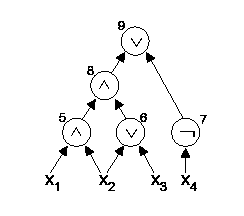
\includegraphics{img/bo/leprikl}
  \caption{Booleovský obvod $C_4$ z príkladu \ref{bo_prikl_le}} \label{bo_obr_lepriklad}
\end{figure}

\begin{definicia}
  Postupnosť booleovských obvodov $\{ C_n\}$ veľkosti $S(n)$ a hĺbky
  $D(n)$ je
  \begin{enumerate}
    \item $\mathcal{U}_E$ - uniformná, ak existuje $DTS\; A$ taký,
    že $L(A)=L_e$ a slová $\langle n,g,p,y\rangle$ akceptuje v čase
    $\log S(n)$
    \item $\mathcal{U}_{E^*}$ - uniformná, ak existuje $ATS\; A$
    taký, že $L(A)=L_e$ a slová $\langle n,g,p,y\rangle$ akceptuje v
    čase $D(n)$ a priestore $\log S(n)$.
  \end{enumerate}
\end{definicia}

Všimnime si, že priestor potrebný na akceptovanie jazyka $L_e$
nezávisí od dĺžky vstupného\linebreak slova, ale od nejakého
podslova vstupného slova. Preto nie je korektné na základe
definície $\mathcal{U}_E$ uniformity písať $L_e\in DTIME(\log
SIZE(C_n))$. Na vyjadrenie tejto situácie zavedieme špeciálne
označenie: $L_e\Subset DTIME(\log SIZE(C_n))$, a podobne pri
$\mathcal{U}_{E^*}$ uniformite:\newline $L_e\Subset
ATIMESPACE(DEPTH(n),log SIZE(C_n))$.

V ďalšom budeme predpokladať, že v jazyku $L_e$, ktorý prislúcha
postupnosti $BO$ $\{ C_n\}$, bude použité ``tesné'' (``bez dier'')
očíslovanie vrcholov t.j. ak má obvod $m$ vrcholov, tak čísla
vrcholov budú z množiny $\{1,\dots ,m\}$ resp. $\{ 0,\dots
,m-1\}$.

\begin{lema}
  \label{bo_lema_uniformity}

  Nech $\{ C_n\}$ je postupnosť $BO$, $L_e$ je jej príslušný
  rozšírený jazyk prepojení, a nech $f(n)\in\Omega(\log SIZE(C_n))$.
  Potom štandardný kód $\langle C_n\rangle$ sa dá vypočítať v
  $DSPACE(f(n))$ práve vtedy, keď $L_e\Subset DSPACE(f(n))$.
\end{lema}

\begin{dokaz}
  Dokážeme obe inklúzie:
  \begin{description}
    \item[``$\Rightarrow$''] Máme $DTS\; A$ generujúci kód $\langle
    C_n\rangle$v priestore $f(n)$. Chceme zostrojiť $DTS\; A'$
    akceptujúci jazyk $L_e$ v rovnakom priestore. $A'$ bude na
    vstupnom slove $\langle n,g,p,y\rangle$ pracovať nasledovne:

    $A'$ najskôr overí, či v obvode $C_n$ existuje vrchol s čislom
    $g$. To urobí tak, že bude simulovať $A$ na vstupe $1^n$, až kým
    nevygeneruje slovo $\langle g,t,a,b$ v štandardom kóde. Ak
    $p=\varepsilon$, overí či $y=t$ (ak nie, tak slovo neakceptuje).
    Ak $p\in\{ L,R\}^+$, tak $A'$ potrebuje overiť, či
    $p$-predchodca vrchola $g$ má číslo $y$. To robí rekurzívne:
    \begin{itemize}
      \item ak $p=Lp'$, tak $A'$ simuluje $A$, až kým nevygeneruje
      $\langle a,t',a',b'\rangle$. Ak $p'=\varepsilon$, overí typ t.j.
      či $t'=y$ (ak nie, tak slovo neakceptuje). Inak opäť simuluje
      $A'$, až kým nevygeneruje $p'$-predchodcu vrchola $a$ atď.
      \item ak $p=Rp'$, tak $A'$ simuluje $A$, až kým
      nevygeneruje $\langle b,t',a',b'\rangle$, a pokračuje podobne
      ako v prvom prípade.
    \end{itemize}
    Na prácu $A'$ nám stačí priestor $f(n)$ (v zmysle $\Subset$ notácie),
    lebo v tomto priestore dokážeme simulovať $A$ a pamätať si jedno
    slovo štandardného kódu.
    \item[``$\Leftarrow$''] Máme $DTS\;A'$ akceptujúci jazyk $L_e$ v
    $\Subset$ priestore $f(n)$. Chceme zostrojiť generátor $A$. Na
    vstupnom slove $1^n$ potrebuje $A$ pre každý vrchol číslo $g$ v
    obvode $C_n$ zistiť jeho typ $t$ a jeho vstupy $a,b$, a potom
    zapísať na výstup štvoricu $\langle g,t,a,b\rangle$. To bude
    robiť nasledovne:

    $A$ bude postupne pre $g=0,1,2,\dots$ a $t=x,0,1,\wedge,\vee,I,\neg$
    simulovať $A'$ na vstupe $\langle n,g,\varepsilon,t\rangle$. Ak
    nejakú takúto štvoricu $A'$ akceptuje, znamená to, že v obvode
    $C_n$ sa nachádza vrchol s číslom $g$ a typom $t$. Na zistenie
    vstupov vrchola $g$ bude $A$ postupne pre $a=0,1,2,\dots$ simulovať
    $A'$ na vstupe $\langle n,g,L,a\rangle$. Ak $A'$ pre nejaké $a$
    akceptuje, zistili sme číslo vrchola, ktorý je ľavým vstupom
    vrchola $g$. Podobne, simulovaním $A'$ na vstupe $\langle
    n,g,R,b\rangle$ pre $b=0,1,2,\dots$, zistíme pravý vstup vrchola
    $g$. Teda $A$ môže na výstup zapísať $\langle g,t,a,b\rangle$.
    Toto bude $A$ vykonávať, až kým pre nejaké $g$ $A'$ neakceptuje
    ani jednu zo štvoríc $\langle n,g,\varepsilon,t\rangle$ pre
    všetky $t\in\{ x,0,1,\wedge,\vee,I,\neg\} $. To znamená, že vrchol s takýmto
    číslom v obvode $C_n$ nie je, a vďaka predpokladu o číslovaní
    vrcholov ``bez dier'' vieme, že $A$ už vygeneroval kódy všetkých
    vrcholov v obvode.

    Na túto prácu stačí $A$ priestor $f(n)$, lebo v tomto prietore
    dokáže simulovať $A'$ a pamätať si nejakú informáciu konštantnej
    dĺžky o práve generovanom vrchole.
  \end{description}
\end{dokaz}

Teraz si ukážeme aké vzťahy sú medzi troma uniformitami
booleovských obvodov, ktoré sme doteraz spomenuli.

\begin{veta}
  Medzi uniformitami platia nasledujúce vzťahy:
  \begin{enumerate}
    \item $\mathcal{U}_E DEPTHSIZE(D(n),S(n))\subseteq\mathcal{U}_{BC}
    DEPTHSIZE(D(n),S(n))$
    \item $\mathcal{U}_E DEPTHSIZE(D(n),S(n))\subseteq\mathcal{U}_{E^*}
    DEPTHSIZE(D(n),S(n))$
    \item Nech $D(n)\geq\log^2 (S(n))$, potom\newline
    $\mathcal{U}_{BC} DEPTHSIZE(D(n),S(n))\subseteq\mathcal{U}_{E^*}
    DEPTHSIZE(D(n),S(n))$
  \end{enumerate}
\end{veta}

\begin{dokaz}
  Dokážeme všetky tri inklúzie:
  \begin{enumerate}
    \item Nech $\{ C_n\}$ je $\mathcal{U}_E$-uniformná postupnosť
    $BO$. Z definície vieme, že príslušný jazyk prepojení $L_e\Subset
    DTIME(\log S(n))$. Zjavne žiadny $DTS$ nepoužije viac priestoru
    ako času, takže $L_e\Subset DSPACE(\log S(n))$. Potom z lemy
    \ref{bo_lema_uniformity} plynie, že štandardný kód $\{ C_n\}$ sa dá
    vypočítať v $DSPACE(\log S(n))$, teda $\{ C_n\}$ je
    $\mathcal{U}_{BC}$-uniformná.
    \item Nech $\{ C_n\}$ je opäť $\mathcal{U}_E$-uniformná, teda
    vieme, že $L_e\Subset DTIME(\log S(n))$. Zrejme\linebreak $L_e\Subset
    DTIMESPACE(\log S(n),\log S(n))$. Keďže $DTS$ je špeciálnym
    prípadom $ATS$, tak $L_e\Subset ATIMESPACE(\log S(n),\log
    S(n))$. Zrejme $D(n)\geq\log S(n)$, teda\newline $L_e\Subset
    DTIMESPACE(D(n),\log S(n))$, čo znamená, že $\{ C_n\}$ je
    $\mathcal{U}_{E^*}$-uniformná.
    \item Nech $\{ C_n\}$ je $\mathcal{U}_{BC}$-uniformná postupnosť booleovských obvodov,
    teda jej štandardný kód vieme vygenerovať v $DSPACE(\log S(n))$. Z
    lemy \ref{bo_lema_uniformity} vieme, že príslušný jazyk\linebreak prepojení $L_e\Subset
    DSPACE(\log S(n))$. Zo simulácie $DTS$ na $ATS$ (veta
    \ref{alter_veta_nspaceatime}) plynie\linebreak $L_e\Subset ATIMESPACE(\log^2 S(n),\log
    S(n))$. Z predpokladu $D(n)\geq\log^2 S(n)$ dostávame $L_e\Subset
    ATIMESPACE(D(n),\log S(n))$, čo znamená, že $\{ C_n\}$ je
    $\mathcal{U}_{E^*}$-uniformná.
  \end{enumerate}
\end{dokaz}

\section{Porovnanie modelov $BO$ a $ATS$}

Prv než prejdeme k samotnému porovnaniu modelov, uvedieme si jeden
normálový tvar booleov\-ských obvodov, ktoré neobsahujú hradlo
negácie. Tento normálový tvar následne využijeme v ďalšej vete.

\begin{lema}
  Pre každý $BO$ $C_n$ existuje ekvivalentný $BO$ $C'_n$ obsahujúci
  len vrcholy typu $\wedge$, $\vee$, ``0'', ``1'', ``x'',
  ``$\overline{x}$'', kde ``$\overline{x}$'' označuje negáciu
  vstupného vrchola ``x''.
\end{lema}

\begin{dokaz}
  Majme daný $BO$ $C_n$. Chceme k nemu skonštruovať $BO$ $C'_n$,
  ktorý nebude obsahovať hradlo $\neg$. Jediným miestom v obvode
  $C'_n$, kde sa môže negácia prejaviť, je na vstupe nahradením
  vstupného vrchola ``x'' jeho negáciou ``$\overline{x}$''.

  Odstránenie hradiel $\neg$ z obvodu bude prebiehať nasledovne.
  Obvod $C_n$ budeme prehľadávať (do šírky) od výstupného vrchola k
  vstupným. Ak narazíme na hradlo $\neg$, budeme rozlišovať šesť
  možných prípadov v závislosti na tom, aký vrchol je vstupom pre
  nájdené hradlo:
  \begin{description}
    \item[$\wedge$ :] Vstupom pre $\wedge$ sú nejaké hodnoty $A,B$.
    Vieme, že platí: $\neg(A\wedge B)=\neg A\vee\neg B$, teda
    vrcholy $\neg,\wedge$ nahradíme vrcholmi $\vee,\neg,\neg$ podľa
    obrázka \ref{bo_obr_nonnegbo}a.
    \item[$\vee$ :] Vstupom pre $\vee$ sú nejaké hodnoty $A,B$.
    Vieme, že platí: $\neg(A\vee B)=\neg A\wedge\neg B$, teda
    vrcholy $\neg,\vee$ nahradíme vrcholmi $\wedge,\neg,\neg$ podľa
    obrázka \ref{bo_obr_nonnegbo}b.
    \item[$\neg$ :] Vstupom pre $\neg$ je nejaká hodnota $A$. Platí $\neg(\neg
    A)=A$, teda vrcholy $\neg,\neg$ z obvodu vynecháme (obr. \ref{bo_obr_nonnegbo}c).
    \item[``0'' :] Vrcholy $\neg$,``0'' nahradíme vrcholom ``1''
    (obr. \ref{bo_obr_nonnegbo}d).
    \item[``1'' :] Vrcholy $\neg$,``1'' nahradíme vrcholom ``0''
    (obr. \ref{bo_obr_nonnegbo}e).
    \item[``x'' :] Vrchol $\neg$ a vstupný vrchol ``x'' nahradíme vstupným
    vrcholom ``$\overline{x}$'' s opačnou hodnotou (obr. \ref{bo_obr_nonnegbo}f).
  \end{description}

  \begin{figure}[!ht]
    \centering
    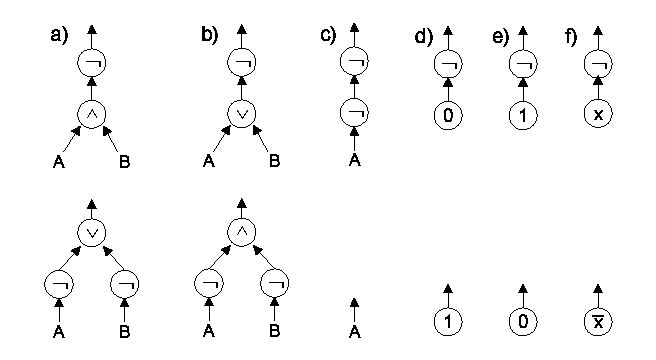
\includegraphics{img/bo/nonnegbo}
    \caption{Modifikácia $BO$ do normálového tvaru} \label{bo_obr_nonnegbo}
  \end{figure}

  V prvých dvoch prípadoch pri modifikácii obvodu opäť využívame
  hradlá $\neg$. Treba si však uvedomiť, že tieto hradlá sú v obvode
  o úroveň nižšie ako pôvodné nahradzované hradlo. Po príslušnej
  úprave obvodu pokračujeme rekurzívne v prehľadávaní obvodu v
  ďalšej úrovni až sa dostaneme k vstupným vrcholom.

  Takto modifikovaný obvod $C'_n$ zrejme akceptuje rovnaký jazyk ako
  $C_n$, lebo každá elementárna modifikácia bola logicky
  ekvivalentná.
\end{dokaz}

\begin{veta}
  Nech $S(n)\geq n$, potom platí:
  \\ $\mathcal{U}_{E^*}DEPTHSIZE(D(n),S(n))\subseteq
  ATIMESPACE(D(n),\log S(n))$.
\end{veta}

\begin{dokaz}
  Nech $\{ C_n\}$ je $E^*$-uniformná postupnosť $BO$ hĺbky $D(n)$ a
  veľkosti $S(n)$ v normálnom tvare z predchádzajúcej lemy, a nech
  $A'$ je $ATS$ akceptujúci príslušný jazyk prepojení $L_e$ v čase
  $D(n)$ a priestore $\log S(n)$. Chceme zostrojiť $ATS$ $A$
  simulujúci $\{ C_n\}$. Uvažujme nejaké slovo $w=a_1\dots a_n\in
  L(\{ C_n\})$ dĺžky $n$ (t.j. $w$ je akceptované $BO$ $C_n$).
  Ukážeme, ako pracuje $A$ na vstupnom slove $w$.

  $A$ uhádne číslo a typ výstupného vrchola $g_{out},t_{out}$. To
  urobí tak, že sa existenčne rozvetví na veľa vetiev a v každej
  vetve na pracovnú pásku zapíše binárne číslo dĺžky najviac $\log
  S(n)$ a nejaký typ vrchola\footnote{Naozaj to bude tak, že pod
  počiatočnou konfiguráciou sa rozvetví binárny strom hĺbky $\log
  S(n)$, pričom pri prechode na nižšiu úroveň $A$ pripíše k už
  vygenerovanému binárnemu číslu jeden bit podľa cesty v binárnom
  strome od koreňa.}. Každá takáto vetva overí svoje hádanie t.j.
  univerzálne spustí proces, v ktorom sa bude simulovať $A'$ na
  vstupe\footnote{$A$ má v každej vetve na pracovnej páske zapísané
  iba $\langle g_{out},t_{out}\rangle $, preto treba ešte vhodne
  dopísať $\varepsilon$. $n$ na pracovnú pásku zapísať nemôžeme,
  lebo jej priestor $\log S(n)$ je na to malý. Nie je však problém
  upraviť $A'$ tak, aby $n$, keďže je kódované unárne, prečítal zo
  vstupnej pásky $A$, kde ja zapísané vstupné slovo $w$ dĺžky $n$.}
  $\langle n,g_{out},\varepsilon,t_{out}\rangle $, teda či vrchol s
  číslom $g_{out}$ a typom $t_{out}$ v obvode $C_n$ existuje. Ak
  taký vrchol existuje, potrebujeme overiť, či je naozaj výstupný,
  teda opäť vo veľkom univerzálnom vetvení simuláciou $A'$
  overujeme, či pre všetky $h\in\{ 0,1\}^*$ také, že $|h|\leq\log
  S(n)$ platí $\langle n,h,L,g_{out}\rangle \not\in L_e$, a zároveň
  $\langle n,h,R,g_{out}\rangle \not\in L_e$ to znamená, že vrchol
  $g_{out}$ nemá nasledovníkov.

  Uvažujme ďalej výpočet na vetve, ktorá úspešne uhádla výstupný
  vrchol. Na pracovnej páske máme zapísané $\langle
  g_{out},t_{out},\varepsilon\rangle $. V nasledujúcom bude $A$
  hádať typy vrcholov, ktoré sú vstupmi $g_{out}$. $A$ sa podľa typu
  $t_{out}$ ($\wedge$ univerzálne, $\vee$ existenčne) rozvetví
  pričom v jednej vetve bude mať na páske zapísané $\langle
  g_{out},L\rangle $ a v druhej $\langle g_{out},R\rangle $.

  Vo všeobecnosti bude mať $A$ na páske zapísané $\langle g,p\rangle $,
  kde $g$ je číslo nejakého vrchola a $p\in\{ L,R\}^*$ je nejaká
  navigačná cesta dĺžky najviac $\log S(n)$. $A$ v tomto prípade
  uhádne typ vrchola $g(p)$ ($p$-predchodca vrchola $g$) a univerzálne
  sa rozvetví na dve vetvy:
  \begin{itemize}
    \item V jednej overí, že hádal správne typ t.j. uhádne číslo
    $p$-predchodcu vrchola $g$ (teda v existenčnom vetvení si $A$
    zapíše na pásku binárne číslo $g(p)$) a overí, že hádal správne,
    teda simuluje $A'$ na vstupe $\langle n,g,p,g(p)\rangle $. Následne overí, že
    pre $p$-predchodcu vrchola $g$ hádal správny typ, teda simuluje
    $A'$ na vstupe $\langle n,g(p),\varepsilon,t_{g(p)}\rangle $.
    \item V druhej vetve pokračuje vo výpočte. To znamená, že podľa
    hádaného typu vrchola $g(p)$ sa ($\wedge$ univerzálne, $\vee$
    existenčne) rozvetví, pričom v jednej vetve si k navigačnej
    ceste $p$ na pásku pripíše $L$ a v druhej si pripíše $R$, teda
    $A$ bude v situácii kedy má na páske zapísané $\langle g,p'\rangle $, kde $p'$
    je v jednom prípade $pL$, v druhom $pR$. V oboch vetvách $A$
    postupuje rovnako ako sme naznačili vyššie.

    V prípade, že typ vrchola $g(p)$ je vstup, $A$ uhádne, ktorý
    i-ty vstup to je a či je typu ``$x_i$'' alebo
    ``$\overline{x}_i$''. Hádanie v univerzálnom vetvení overí, teda
    v jednej vetve simuluje $A'$ na vstupe
    $\langle n,g(p),\varepsilon,x_i\rangle $ resp.
    $\langle n,g(p),\varepsilon,\overline{x}_i\rangle $ a v druhej vetve výpočet
    končí s tým, že
    \begin{itemize}
      \item ak je vstup typu ``$x_i$'', tak $A$ akceptuje, ak $a_i=1$
      (neakceptuje, ak $a_i=0$)
      \item ak je vstup typu ``$\overline{x}_i$'', tak $A$
      akceptuje, ak $a_i=0$ (neakceptuje, ak $a_i=1$)
    \end{itemize}
  \end{itemize}

  Uvažujme teraz prípad, že dĺžka navigačnej cesty $p$ na páske
  dosiahne hranicu $\log S(n)$. To je problém, pretože priestor
  pracovnej pásky $A$ je ohraničený na $O(\log S(n))$ a naviac pri
  väčšej dĺžke $p$ by sme už ani nemohli jednoducho overovať hádanie
  simuláciou $A'$, lebo slová jazyka $L_e$ sú definované s
  navigačnou cestou dĺžky najviac $\log S(n)$. V tomto prípade
  postupojeme nasledovne:

  $A$ má na páske zapísané $\langle g,p\rangle $, pričom $|p|=\log
  S(n)$. V existenčnom vetvení uhádne číslo $h$ a typ $t_h$ vrchola
  $g(p)$ a univerzálne
  \begin{itemize}
    \item overí či $\langle n,g,p,h\rangle \in L_e$ a $\langle n,h,\varepsilon,t_h\rangle \in
    L_e$
    \item pokračuje vo výpočte, pričom na páske má zapísané
    $\langle h,t_h,\varepsilon\rangle $, teda sme v podobnej situácii, ako sme
    boli na začiatku po uhádnutí výstupného vrchola.
  \end{itemize}

  Z konštrukcie by malo byť vidieť, že skonštruovaný $ATS$ $A$
  naozaj akceptuje práve slová z jazyka $L(\{ C_n\})$.

  Zamyslime sa teraz nad časovou a priestorovou zložitosťou $A$:
  \begin{itemize}
    \item Uhádnutie výstupného vrchola trvá čas $\log S(n)\leq D(n)$.
    \item Ak má $A$ na páske zapísanú cestu $p$ dĺžky menšej ako $\log
    S(n)$, tak $A$ sa v hlavnom výpočte (hádanie ďalšej úrovne
    $C_n$) posunie v konštantnom čase vďaka tomu, že pri
    rozvetvovaní stačí na páske predĺžiť cestu $p$ o $L$ resp. $R$.
    Všetky dlhé hádania a overovania sa robia v bočných vetvách
    výpočtu, a teda ich netreba do celkového času zarátať. Musíme si
    však uvedomiť, že tieto bočné vetvy sú dlhé najviac $D(n)$, lebo
    v nich $A$ buď háda, teda zapisuje na pásku (ale sú to vždy informácie
    dĺžky najviac $D(n)$), alebo simuluje $A'$, ten však z definície
    pracuje v čase $O(D(n))$.
    \item Každú $(\log S(n))$-tú úroveň výpočtu dosiahne dĺžka $p$
    hranicu $\log S(n)$. $A$ vtedy musí znova hádať v hlavnom
    výpočte číslo vrchola - na to spotrebuje čas $O(\log S(n))$.
    Keďže obvod má hĺbku $D(n)$, takýchto situácií sa počas výpočtu
    vyskytne $\frac{D(n)}{\log S(n)}$ krát. Na riešenie všetkých týchto
    situácií spotrebuje $A$ čas $O(\frac{D(n)}{\log S(n)} \log S(n))=O(D(n))$.
    \item Na koncoch jednotlivých vetiev výpočtu pri zisťovaní
    hodnoty i-teho vstupu musí $A$ presunúť hlavu nad tento symbol.
    Pri dĺžke vstupu $n$ by sme na túto operáciu potrebovali čas $O(n)$,
    čo je priveľa. Preto budeme uvažovať, že $ATS$ $A$ má rýchly
    prístup na vstupnú pásku, teda nám bude stačiť čas $\log n$, čo
    je menej ako $D(n)$ vďaka predpokladu $S(n)\leq n$ zo znenia
    vety.
    \item Počas celého výpočtu bolo na páske zapísané číslo nejakého
    vrchola dĺžky najviac $\log S(n)$, navigačná cesta dĺžky najviac
    $\log S(n)$ a typ vrchola konštantnej dĺžky, čo celkovo dáva
    nároky na priestor $O(\log S(n))$.
  \end{itemize}
  Z uvedeného vyplýva, že sme konštrukciou $ATS$ $A$ splnili
  požiadavky na korektnosť akceptácie ako aj na časovú a priestorovú
  zložitosť.
\end{dokaz}

\begin{veta}
Nech $S(n)\geq\log n$, potom pre vhodnú konštantu $k$ platí:\newline
$ATIMESPACE(T(n),S(n))\subseteq\mathcal{U}_E
DEPTHSIZE(T(n),k^{S(n)})$
\end{veta}

\begin{dokaz}
  K danému $ATS\;A$ chceme zostrojiť postupnosť $BO$ $\{ C_n\}$
  akceptujúcu jazyk $L(A)$. Skôr ako začneme konštruovať $\{ C_n\}$
  zamyslime sa nad tým ako vyzerá výpočet na $ATS$.

  Predstavme si úplný strom konfigurácií $ATS\;A$ na nejakom
  vstupnom slove $w$. Na výpočet $A$ sa môžme pozerať aj ako na
  vyhodnocovanie tohto stromu zdola. Každý vrchol reprezentujúci
  akceptačnú konfiguráciu na konci nejakej vetvy v strome
  konfigurácií ohodnotíme 1. Ostatné vrcholy na konci vetiev ako aj
  nekonečné vetvy ohodnotíme 0. Každý vrchol reprezentujúci
  univerzálnu konfiguráciu ohodnotíme 1 práve vtedy, keď všetci jeho
  synovia majú hodnotu 1. Vrchol reprezentujúci existenčnú
  konfiguráciu ohodnotíme 1 práve vtedy, keď aspoň jeden z jeho
  synov má hodnotu 1. Vstupné slovo $w$ bude $A$ akceptovať práve
  vtedy, keď koreň stromu (vrchol reprezentujúci počiatočnú
  konfiguráciu $A$ na slove $w$) ohodnotíme 1.

  Uvažujme teraz $ATS\;A$ v nasledovnom normálovom tvare:\newline
  $A$ pracuje s binárnou vstupnou aj pracovnou abecedou, $A$ používa
  rýchly prístup na vstupnú pásku (t.j. $A$ má špeciálnu pásku dĺžky
  $\log n$, na ktorú keď v binárnom kódovaní zapíše číslo $j$,
  dostane sa k $j$-temu symbolu na vstupe), úplný strom konfigurácií
  je binárny a v každej vetve tohto stromu môže $A$ čítať vstup iba
  raz, a to na konci (t.j. $A$ má špeciálne čítacie stavy $q^0$ a
  $q^1$, do ktorých sa dostane na konci výpočtu vetvy, pričom v
  stave $q^0$ očakáva na vstupe\footnote{na jednej pozícii vstupu
  určenej číslom na špeciálnej páske} 0 (ak je na vstupe naozaj 0,
  tak akceptuje, ak je tam 1, neakceptuje) a v $q^1$ očakáva na
  vstupe 1).

  Pozrime sa teraz na úplný strom konfigurácií $A$. Má $T(n)$
  úrovní, pričom v nultej úrovni bude jediný vrchol reprezentujúci
  počiatočnú konfiguráciu. Hľadaný $BO$ $C_n$ akceptujúci vstupné
  slovo $w$ dĺžky $n$ bude vyzerať veľmi podobne. Každému vrcholu v
  úplnom strome konfigurácií zodpovedá jeden vrchol v obvode $C_n$.

  Vrcholu na úrovni $t$, ktorý reprezentuje
  konfiguráciu\footnote{Uvažujeme tu konfiguráciu bez vstupu, lebo
  každý FORKovaný výpočet používa len jeden symbol zo vstupu, takže
  vstup v konfigurácii de facto nepotrebujeme. Na druhej strane
  veľmi užitočná v konfigurácii je informácia o špeciálnej páske
  určujúcej ktorý symbol sa má čítať na konci výpočtu.} $c$ v strome
  konfigurácií zodpovedá v obvode $C_n$ vrchol s číslom $f(t,c)$,
  kde $f:N\times N\rightarrow N$ je funkcia zachovávajúca tesné
  očíslovanie vrcholov, pričom
  \begin{itemize}
    \item ak $c$ je univerzálna konfigurácia, tak vrchol $f(t,c)$ je
    typu $\wedge$
    \item ak $c$ je existenčná konfigurácia, tak vrchol $f(t,c)$ je
    typu $\vee$
    \item ak $c$ je čítacia konfigurácia so stavom $q^0$ a na
    špeciálnej páske je zapísané číslo $j$, tak vrchol $f(t,c)$ je
    typu\footnote{Ak $A$ očakáva na vstupe 0 a naozaj tam 0 je, tak
    hradlo $\neg$ dostane na vstup 0 a na výstup pošle 1, čo signalizuje,
    že $A$ očakával správne. Naopak ak je na vstupe 1, tak hradlo $\neg$
    pošle na výstup 0, čo signalizuje, že $A$ sa mýlil. Analogicky to
    funguje pre stav $q^1$ a hradlo $I$.} $\neg$ a jeho vstupom je
    $j$-ty bit vstupného slova $w$
    \item ak $c$ je čítacia konfigurácia so stavom $q^1$ a na
    špeciálnej páske je zapísané číslo $j$, tak vrchol $f(t,c)$ je
    typu $I$ a jeho vstupom je $j$-ty bit vstupného slova $w$
    \item ak $c$ je akceptačná konfigurácia ale nie je čítacia, tak
    vrchol $f(t,c)$ je typu ``1''
    \item ak $c$ je odmietacia konfigurácia ale nie je čítacia, tak
    vrchol $f(t,c)$ je typu ``0''
  \end{itemize}

  \begin{figure}[!ht]
    \centering
    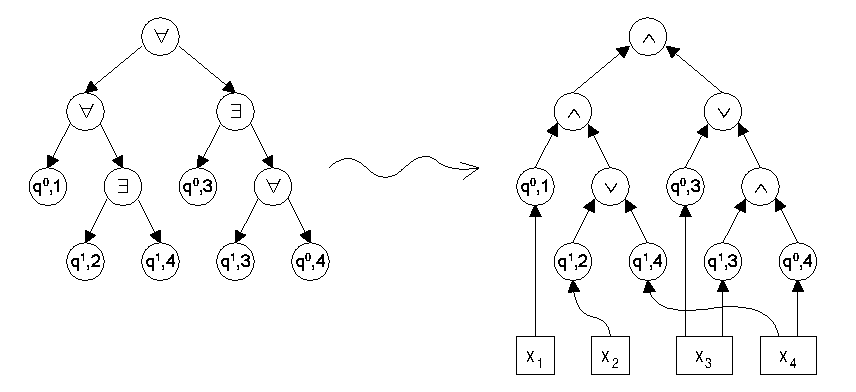
\includegraphics{img/bo/atsbo}
    \caption{Konštrukcia $BO$ k $ATS$} \label{bo_obr_atsbo}
  \end{figure}

  Vstupnými vrcholmi pre vrchol $f(t,c)$ sú vrcholy s číslami
  $f(t+1,c_1)$ a $f(t+1,c_2)$ pričom platí $c\underset{A}{\vdash}
  c_1$ a $c\underset{A}{\vdash} c_2$ (obr. \ref{bo_obr_atsbo}).

  Takto zostrojený obvod $C_n$ pracuje presne tak ako výpočet $ATS$,
  ktorý sme opísali na začiatku dôkazu. Teda príslušná postupnosť
  $BO$ $\{ C_n\}$ zrejme akceptuje jazyk $L(A)$.

  Pozrime sa ešte na miery zložitosti obvodu $C_n$. Obvod sme
  zostrojili ``jedna k jednej'' vzhľadom na úplný strom konfigurácií
  $ATS\;A$. Z toho plynie, že $DEPTH(C_n)=T(n)$. $SIZE(C_n)$
  zodpovedá počtu vrcholov v strome konfigurácií. Keďže do
  konfigurácií nezahŕňame vstup, tak počet všetkých možných
  konfigurácií je $k^{S(n)}$ pre vhodné $k$. V zásade sa môže stať, že v úplnom
  strome konfigurácií máme v dvoch rôznych vetvách vrcholy
  reprezentujúce rovnakú konfiguráciu, čo by mohlo spôsobiť, že
  počet vrcholov, a teda aj veľkosť $C_n$ by bola rádovo väčšia ako
  $k^{S(n)}$. Ak ale uvažujeme výpočet $ATS$ ako FORKovanie
  procesov, tak nie je potrebné, aby boli spustené dva rovnaké
  procesy. Takže ak chce $ATS$ spustiť proces, ktorého kópia už
  beží, tak tento duplicitný proces iba odkážeme na rovnaký už
  bežiaci proces. To v booleovskom obvode znamená jedno prepojenie
  medzi hradlami. Takže v konečnom dôsledku môžme uvažovať opäť
  akýsi normálový tvar $ATS$, ktorý bude mať v úplnom strome
  konfigurácií všetky konfigurácie disjunktné, a teda
  $SIZE(C_n)=O(k^{S(n)})$.
\end{dokaz}
